\section{Analyzing ESBL E. coli isolates from patients of the University hospital Basel}
\subsection{Selection of samples suitable for our analysis}
The phylogenetic tree of all samples is shown in Figure \ref{figure:panX}. This tree revealed that many patients were infected with different ESBL \textit{E. coli} strains over time suggesting reinfection rather than in-patient evolution. This was visible in the tree when samples of one patient mapped on different branches. Interestingly some samples from different patients mapped on the same branch which suggests that those patients were infected from the same outbreak. The selected patients and the MICs of their ESBL \textit{E. coli} samples is shown in Table \ref{table:samples}.

\begin{figure}[H]
	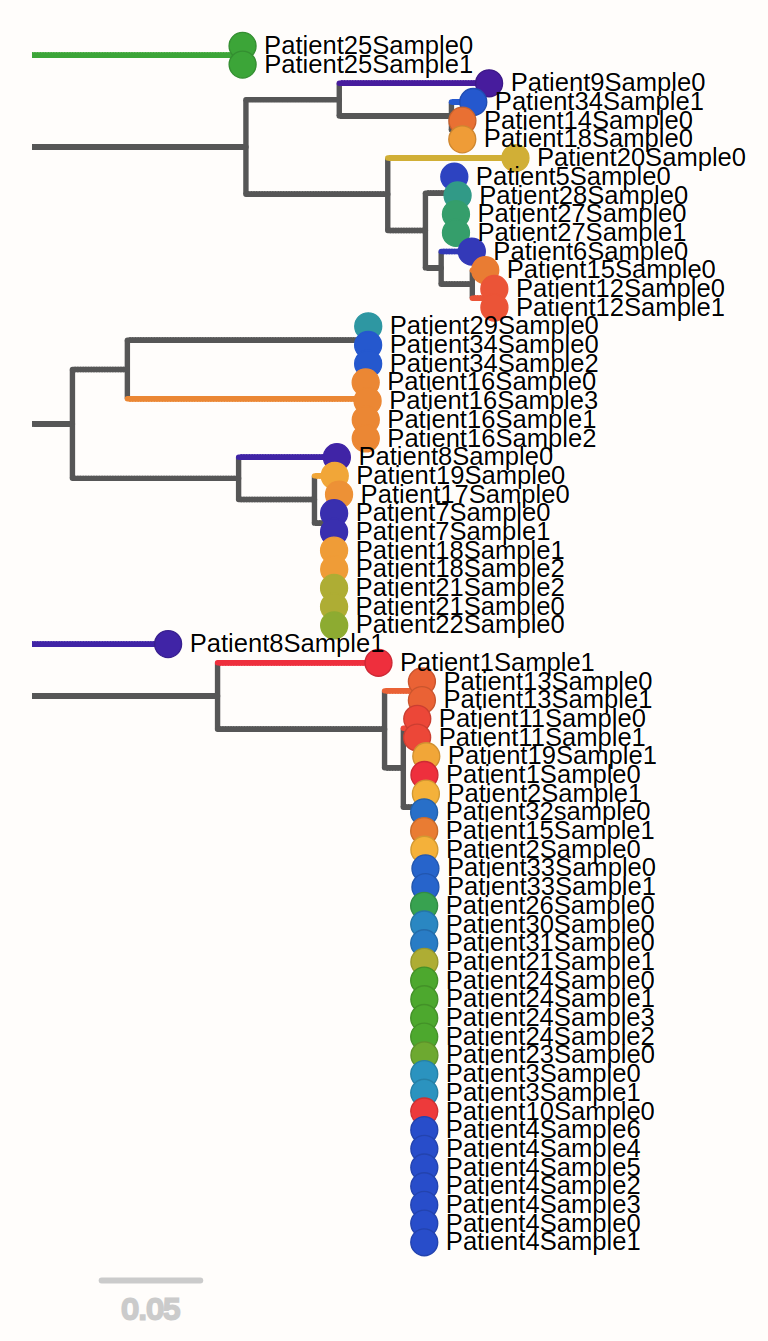
\includegraphics[scale=0.2]{181205_panXtree_overview.png}
	\caption{Phylogenic tree built for every ESBL \textit{E. coli} sample}
	\label{figure:panX}
\end{figure}

\begin{table}[H]
	\begin{tabularx}{\textwidth}{|cccLL|}
		\hline
		Patient                   & Sample                   & Sample date                     & MIC cefepim {[}\textmu g/ml{]} & MIC ceftazidime {[}\textmu g/ml{]} \\ \hline
		\rowcolor[HTML]{FFCE93} 
		{\color[HTML]{000000} 12} & {\color[HTML]{000000} 0} & {\color[HTML]{000000} 09/09/14} & {\color[HTML]{000000} 4}                      & {\color[HTML]{000000} 0.75}                       \\
		& 1                        & 05/12/14                        & 12                                            & 2                                                 \\ \hline
		\rowcolor[HTML]{FFCE93} 
		16                        & 0                        & 22/06/12                        & 8                                             & 2                                                 \\
		& 1                        & 18/07/13                        & 48                                            & 8                                                 \\
		& 2                        & 01/11/13                        & 32                                            & 12                                                \\ \hline
		\rowcolor[HTML]{FFCE93} 
		24                        & 0                        & 02/05/11                        & 4                                             & 1.5                                               \\
		& 1                        & 08/15/11                        & 16                                            & 1.5                                               \\
		& 2                        & 11/28/11                        & 3                                             & 1                                                 \\ \hline
		25                        & 0                        & 15/04/11                        & 64                                            & 192                                               \\
		\rowcolor[HTML]{FFCE93} 
		& 1                        & 22/08/11                        & 6                                             & 6                                                 \\ \hline
		33                        & 0                        & 26/09/14                        & 6                                             & 6                                                 \\
		\rowcolor[HTML]{FFCE93} 
		& 1                        & 29/01/15                        & 1                                             & 1.5                                               \\ \hline
	\end{tabularx}
	\caption{Selected patients and the MIC of cefepim and ceftazidime for their ESBL \textit{E. coli} samples. Samples highlighted in orange were chosen as reference genomes.}
	\label{table:samples}
\end{table}
\subsection{Identification of mutations}
For patient 12,16 and 24 we chose sample 0, for patient 25 and 33 we chose sample 1 for building a reference genome. The selected samples are stained orange in Table \ref{table:samples}.

\subsection{Identified mutations for the selected sample series}
\subsubsection{Patient 12}
Our bioinformatic pipeline revealed two positions where the dominant nucleotide changed (also referred as SNPs) between the samples of patient 12. For those positions, shown in Table \ref{table:patient12}, no annotation was available. 
\begin{table}[H]
	\begin{tabularx}{\linewidth}{|cccLL|}
		\hline
		\#SNP & Contig & Position & \multicolumn{2}{l|}{Nucleotide in Sample:} \\
		&        &          & 0         & \multicolumn{1}{l|}{1}    \\ \hline
		1 & 0 & 880249  & C & A \\ \hline
		2 & 0 & 4256761 & A & T \\ \hline
	\end{tabularx}
	\caption{Positions of SNPs between samples of patient 12}
	\label{table:patient12}
\end{table} 
\subsubsection{Patient 16}
In Table \ref{table:patietn16} we show the positions of SNPs between samples of patient 16. Our pipeline found six genes and one promoter affected by the SNPs. The affected genes are shown in Table \ref{table:pat16annot} and the affected promoter in Table \ref{table:pat16_prom}. This promoter annotation was obtained from the EcoCyc promoter sequences. 
\begin{table}[H]
	\begin{tabularx}{\linewidth}{|cccLLL|}
		\hline
		\#SNP & Contig & Position & \multicolumn{3}{l|}{Nucleotide in Sample:} \\
		&        &          & 0     & 1     & \multicolumn{1}{l|}{2}    \\ \hline
		1     & 0      & 109928   & C     & A     & \multicolumn{1}{l|}{C}    \\ \hline
		2     & 0      & 1895312  & A     & C     & \multicolumn{1}{l|}{A}    \\ \hline
		3     & 0      & 2101128  & G     & -     & \multicolumn{1}{l|}{-}    \\ 
		&        & 2101129  & C     & -     & \multicolumn{1}{l|}{-}    \\ 
		&        & 2101130  & A     & -     & \multicolumn{1}{l|}{-}    \\ \hline
		4     & 0      & 2375277  & C     & T     & \multicolumn{1}{l|}{C}    \\ \hline
		5     & 0      & 3797984  & A     & G     & \multicolumn{1}{l|}{A}    \\ \hline
		6     & 0      & 4200032  & T     & C     & \multicolumn{1}{l|}{T}    \\ \hline
		7     & 0      & 4353560  & G     & C     & \multicolumn{1}{l|}{G}    \\ \hline
		8     & 0      & 5112127  & G     & T     & \multicolumn{1}{l|}{G}    \\ \hline
		9     & 0      & 55597    & A     & G     & \multicolumn{1}{l|}{G}    \\ \hline
		10    & 0      & 922702   & G     & A     & \multicolumn{1}{l|}{G}    \\ \hline
		11    & 0      & 1133762  & C     & T     & \multicolumn{1}{l|}{T}    \\ \hline
		12    & 0      & 1549518  & T     & G     & \multicolumn{1}{l|}{G}    \\ \hline
		13    & 0      & 2016331  & A     & C     & \multicolumn{1}{l|}{A}    \\ \hline
		14    & 0      & 2101129  & C     & -     & \multicolumn{1}{l|}{-}    \\ 
		&        & 2101130  & A     & -     & \multicolumn{1}{l|}{-}    \\ \hline
		15    & 0      & 3920934  & A     & G     & \multicolumn{1}{l|}{A}    \\ \hline
		16    & 0      & 4333944  & C     & T     & \multicolumn{1}{l|}{T}    \\ \hline
		17    & 0      & 4459680  & C     & -     & \multicolumn{1}{l|}{C}    \\ 
		&        & 4459681  & C     & -     & \multicolumn{1}{l|}{C}    \\ \hline
		18    & 0      & 4459684  & G     & -     & \multicolumn{1}{l|}{G}    \\ 
		&        & 4459685  & A     & -     & \multicolumn{1}{l|}{A}    \\ 
		&        & 4459686  & A     & -     & \multicolumn{1}{l|}{A}    \\ 
		&        & 4459687  & G     & -     & \multicolumn{1}{l|}{G}    \\ 
		&        & 4459688  & A     & -     & \multicolumn{1}{l|}{A}    \\ 
		&        & 4459689  & G     & -     & \multicolumn{1}{l|}{G}    \\ \hline
		19    & 0      & 4459692  & A     & -     & \multicolumn{1}{l|}{A}    \\ 
		&        & 4459693  & G     & -     & \multicolumn{1}{l|}{G}    \\ \hline
		20    & 0      & 4459695  & G     & -     & \multicolumn{1}{l|}{G}    \\ \hline
		21    & 0      & 4459697  & T     & -     & \multicolumn{1}{l|}{T}    \\ \hline
	\end{tabularx}
	\caption{Positions of SNPs in the sample of patient 16.}
	\label{table:patietn16}
\end{table}
\begin{table}[H]
	\begin{tabularx}{\linewidth}{|ccLLccc|}
		\hline
		\#SNP & Gene          & Product                                  & Type and position in gene      & \multicolumn{3}{l|}{Amino acid in Sample:} \\
		&               &                                          &                        & 0   & 1               & 2               \\ \hline
		1     & \textit{ortT} & Orphan toxin OrtT                        & Missense, 44           & P   & T               & P               \\ \hline
		2     & \textit{scrY} & Sucrose Porin                            & Missense, 104          & L   & V               & L               \\ \hline
		3     & \textit{cpdA} & Phosphodiesterase CpdA                   & In-frame deletion, 162 & L   & -   & -   \\ \hline
		4     & \textit{rpoB} & DNA-directed RNA polymerase subunit beta & Missense, 113          & V   & I               & V               \\ \hline
		5     & \textit{ftsQ} & Cell division protein FtsQ               & Missense, 207          & K   & R               & K               \\ \hline
		4     & \textit{recR} & Recombination protein RecR               & Missense, 40           & M   & T               & M               \\ \hline
		5     & \textit{hcxA} & Hydoxycarboxylate dehydrogenase A        & Missense, 332          & R   & G               & R               \\ \hline
		6     & \textit{ribA} & GRP cyclohydrolase-2                     & Missense, 68           & F   & L               & L               \\ \hline
	\end{tabularx}
	\caption{Genes affected by the SNPs found in the samples of patient 16.}
	\label{table:pat16annot}  
\end{table}
\begin{table}[H]
	\begin{tabular}{|lll|}
		\hline
		\#SNP & Transcription unit & Next upstream gene \\ \hline
		16    & fes-ybdZ-entF-fepE & \textit{fepA}      \\ \hline
	\end{tabular}
	\caption{Identified promoter affected by a SNP in the samples of patient 16.}
	\label{table:pat16_prom}
\end{table}
The fepA promoter sequence affected by a SNP is shown in the Alignment \ref{figure:alignment}. The polymorph position, marked with a red box, was found in the binding site of the \textsigma 70 transcription factor.  
\begin{texshade}{pat16fepa.aln}
	\showruler{1}{top}
		\feature{bottom}{1}{24..29}{fill:-}{-35}
	\feature{bottom}{1}{48..53}{fill:-}{-10}
	\feature{top}{1}{60..60}{fill:$\downarrow$}{Start of $\sigma$70 binding site}
	\hideconsensus
	\frameblock{1}{80..80}{Red[1pt]}
	\showcaption{This alignment shows the SNP in the fepA promotor. Positions marked with dashed lines are the recognition sites for $\sigma$70 factor.}
	\label{figure:alignment}
\end{texshade}
\subsubsection{Patient 24}
Identified SNPs in the samples of patient 24 are show in Table \ref{table:pat24}, the affected genes are shown in Table \ref{table:pat24_ann}.
\begin{table}[h]
	\begin{tabularx}{\linewidth}{|cccLLL|}
		\hline
		\#SNP & Contig & Position & \multicolumn{3}{l|}{Nucleotide in Sample:} \\
			&        &          & 0     & 1     & \multicolumn{1}{l|}{2}    \\ \hline
	1     & 0      & 50032    & G            & A            & G            \\ \hline
	2     & 0      & 418564   & C            & T            & C            \\ \hline
	3     & 0      & 2048961  & A            & C            & C            \\ \hline
	4     & 0      & 2319554  & T            & A            & A            \\ \hline
	5     & 0      & 3444478  & T            & C            & T            \\ \hline
	6     & 0      & 4063226  & G            & T            & T            \\ \hline
	\end{tabularx}
	\caption{Positions of SNPs in the samples of patient 24.}
	\label{table:pat24}
\end{table}

\begin{table}[H]
	\begin{tabularx}{\linewidth}{|ccLLccc|}
		\hline
		\#SNP & Gene          & Product                                  & Type and position in gene      & \multicolumn{3}{l|}{Amino acid in Sample:} \\
		&               &                                          &                        & 0   & 1               & 2               \\ \hline
		1     & \textit{atl}     & DNA base-flipping protein                                  & Missense, 87      & V           & M           & V           \\ \hline
		2     & \textit{imm\_2}  & Colicin-E7 immunity protein                                & Missense, 69      & K           & E           & K           \\ \hline
		3     & \textit{lldR\_2} & Lactate Dehydrogenase regulatory protein & Missense, 44      & I           & S           & S           \\ \hline
		4     & \textit{dctM\_2} & TRAP transporter large permease protein                                                        & Missense, 112     & T           & S           & S           \\ \hline
		5     & \textit{dltA}    & D-alanine--D-alanyl carrier protein ligase subunit 1           & Missense, 692     & E           & G           & E           \\ \hline
		6     & \textit{fnr}     & Fumarate and nitrate reduction regulatory protein          & Missense, 31      & C           & F & F  \\ \hline    
	\end{tabularx}
	\caption{Genes affected by the SNPs found in the samples of patient 24.}
	\label{table:pat24_ann}
\end{table}

\subsubsection{Patient 25}
The identified SNPs between the samples of patient 25 are shown in Table \ref{table:pat25}. The genes affected by those SNPs are shown in Table \ref{table:pat25_ann}.

\begin{table}[H]
	\begin{tabularx}{\linewidth}{|cccLL|}
		\hline
		\#SNP & Contig & Position & \multicolumn{2}{l|}{Nucleotide in Sample:} \\
		&        &          & 0         & \multicolumn{1}{l|}{1}    \\ \hline
	1 & 0 & 396325   & G & A \\ \hline
	2 & 0 & 396846  & G & A \\ \hline
	3 & 0 & 1996537 & - & C \\ 
	&   & 1996538 & - & C \\ 
	&   & 1996539 & - & G \\ 
	&   & 1996540 & - & T \\ 
	&   & 1996541 & - & A \\ 
	&   & 1996542 & - & C \\ 
	&   & 1996543 & - & C \\ 
	&   & 1996544 & - & A \\ 
	&   & 1996545 & - & G \\ 
	&   & 1996546 & - & C \\ 
	&   & 1996547 & - & T \\ 
	&   & 1996548 & - & G \\ \hline
	4 & 0 & 3743644 & A & G \\ \hline
	5 & 0 & 4785433 & G & A \\ \hline
	6 & 0 & 4785439 & G & A \\ \hline
	\end{tabularx}
	\caption{Positions of SNPs in the samples of patient 25.}
	\label{table:pat25}
\end{table} 

\begin{table}[H]
	\begin{tabularx}{\linewidth}{|ccLLcc|}
		\hline
	\#SNP & Gene          & Product                                 & Type and position & \multicolumn{2}{l|}{Amino acid Sample:} \\
	&               &                                         &                   & 0                  & 1                  \\ \hline
	1     & \textit{ompR} & Transcriptional regulatory protein OmpR & Missense, 146     & R                  & H                  \\ \hline
	2     & \textit{envZ} & Osmolarity sensor protein EnvZ          & Missense, 84      & G                  & E                  \\ \hline
	3     & \textit{rfbD} & dTDP-4-dehydrorhamnose reductase        & \multicolumn{3}{l|}{Frameshift deletion, 148-295}            \\ \hline
	\end{tabularx}
	\caption{Genes affected by the SNPs found in the samples of patient 25.}
	\label{table:pat25_ann}
\end{table}

\subsubsection{Patient 33}
Only three SNPs were found for the samples of patient 33, they are shown in Table \ref{table:pat33} with their annotation in Table \ref{table:pat33_ann}.
\begin{table}[h]
	\begin{tabularx}{\linewidth}{|cccLL|}
		\hline
		\#SNP & Contig & Position & \multicolumn{2}{l|}{Nucleotide in Sample:} \\
		&        &          & 0         & \multicolumn{1}{l|}{1}    \\ \hline
		1 & 0 & 4008745 & A & T \\ \hline
		2 & 0 & 4675092 & T & A \\ \hline
		3 & 0 & 1996537 & A & C \\ \hline
	\end{tabularx}
	\caption{Positions of SNPs in the samples of patient 25.}
	\label{table:pat33}
\end{table} 
\begin{table}[H]
	\begin{tabularx}{\linewidth}{|ccLLcc|}
		\hline
		\#SNP & Gene          & Product                           & Type and position & \multicolumn{2}{l|}{Amino acid Sample:} \\
		&               &                                   &                   & 0                  & 1                  \\ \hline
		1     & \textit{cydD} & ATP-binding/permease protein CydD & Missense, 368     & Q                  & L                  \\ \hline
		2     & \textit{vnfA} & Nitrogen fixation protein VnfA    & Missense, 169     & N                  & I                  \\ \hline
	\end{tabularx}
	\caption{Genes affected by the SNPs found in the samples of patient 33.}
	\label{table:pat33_ann}
\end{table}
\subsection{Copynumbers of ESBL genes}
Next to the reference genomes we also hybrid-assemblied and annotated the other samples of the selected sample series. This allowed us to see, if the copy numbers of ESBL genes increased while resistance evolved. The copy numbers of three ESBL genes shown in Table \ref{table:copynumers}. For four out of five patients the copy number remained very similar. Sometimes the ESBL gene was replaced by a different ESBL gene. Only the sample series of patient 33 showed an increase of ESBL genes while resistance evolved. Sample 0 of patient 33 had 9 copies of CTX-M-1 while sample 1 only had one. 
\begin{table}[H]
	\begin{tabularx}{\linewidth}{|ccLLL|}
		\hline
		Patient & Sample & \multicolumn{3}{l|}{Copies of genes coding for textbeta-lactamase} \\
		&        & CTX-M-1                & OXA-1                & TEM                \\ \hline
		12      & 0      & 1                      & 0                    & 0                  \\ \hline
		12      & 1      & 1                      & 0                    & 0                  \\ \hline
		16      & 0      & 2                      & 0                    & 1                  \\ \hline
		16      & 1      & 2                      & 0                    & 1                  \\ \hline
		16      & 2      & 1                      & 0                    & 1                  \\ \hline
		24      & 0      & 1                      & 0                    & 2                  \\ \hline
		24      & 1      & 1                      & 0                    & 2                  \\ \hline
		24      & 2      & 0                      & 0                    & 3                  \\ \hline
		25      & 0      & 1                      & 1                    & 0                  \\ \hline
		25      & 1      & 1                      & 1                    & 0                  \\ \hline
		33      & 0      & 9                      & 0                    & 1                  \\ \hline
		33      & 0      & 1                      & 1                    & 0                  \\ \hline		
	\end{tabularx}
	\label{table:copynumers}
	\caption{Copy number of ESBL genes per sample.}
\end{table}
Studying the short-reads of sample 0  from patient 33 mapped to the assembly from sample 1 revealed that the coverage for sample 0 was very high for a region of 17 kilo base-pairs (kbp). In this region the genes coding for \textbeta lactamase CTX-M-1 (\textit{bla\_2}) was located. This increased coverage, the genes located within this region and the GC-content is shown in Figure \ref{figure:coverage}. This confirmed that the copy number of the gene coding for CTX-M-1 is higher in sample 0.

\begin{figure}[H]
	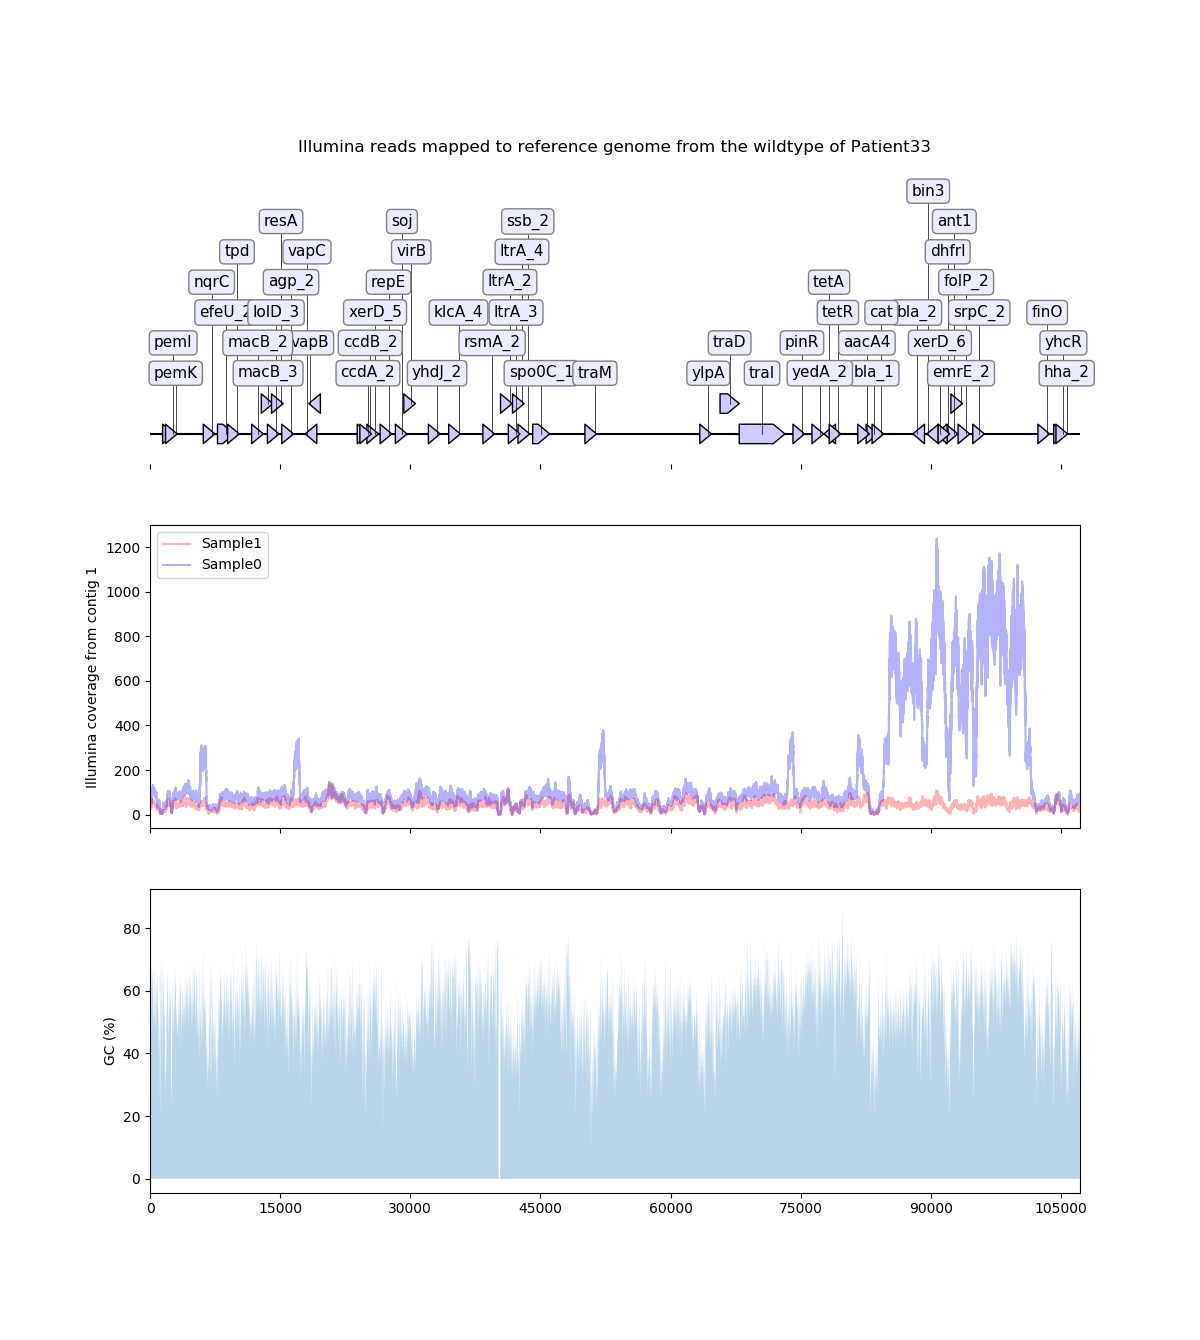
\includegraphics[scale=0.3]{coverage_pat33.png}
	\caption{Upper figure: Annotation of the whole plasmid. Middle figure: Coverage of the illumina sequencing data from sample 0 (resistant sample) and sample 1 (susceptible sample). Bottom figure: GC content.}
	\label{figure:coverage}
\end{figure}

\section{Morbidostat experiments}
Table \ref{table:vial_modes} shows which ESBL \textit{E. coli} strain was cultured in which vial, with which mode. 
\begin{table}[H]
	\begin{tabular}{|c c c|}	
		\hline
		Vial & Strain & Mode \\
		\hline
		1 & pEU26\_OXA & continuous \\
		\hline
		2 & pEU26\_OXA & continuous \\
		\hline
		3 & pEU23\_OXA & continuous \\
		\hline
		4 & pEU23\_OXA & continuous \\
		\hline
		5 & pEU23\_OXA & continuous \\
		\hline
		8 & pEU26\_OXA & continuous \\
		\hline
		9 & pEU23\_OXA & fixed OD \\
		\hline
	\end{tabular}
	\quad
	\begin{tabular}{|c c c|}	
		\hline
		Vial & Plasmid & Mode \\
		\hline
		1 & pEU26\_OXA & continuous \\
		\hline
		2 & pEU23\_OXA & continuous \\
		\hline
		3 & pEU22\_CTX-M-1 & continuous \\
		\hline
		4 & pEU22\_CTX-M-1 & continuous \\
		\hline
		5 & pEU22\_CTX-M-1 & continuous \\
		\hline
		7 & K12 & continuous \\
		\hline
		8 & pEU22\_CTX-M-1 & fixed OD \\
		\hline
		9 & pEU26\_OXA & fixed OD \\
		\hline
		10 & pEU26\_OXA & fixed OD \\
		\hline
	\end{tabular}
	\caption{Left table: Experiment 01, right table: Experiment 02}
	\label{table:vial_modes}
\end{table}
\subsection{Contamination analysis}
\begin{table}[H]
	\begin{tabularx}{\linewidth}{|LLLLL|}
		\hline
		Stocked strain    & Total reads & Reads mapped to \textit{Bacillus cereus} & Reads mapped to \textit{E. coli} & \% of reads mapped to \textit{Bacillus cereus ATCC 14579} \\ \hline
		pEU22\_CTX & 3810442     & 16496                                                     & 3803789                                           & 0.43                                                            \\ \hline
		pEU23\_OXA & 4329090     & 18499                                                     & 4322708                                           & 0.43                                                            \\ \hline
		pEU26\_OXA & 4040571     & 17629                                                     & 4036167                                           & 0.44                                                            \\ \hline
		K-12 MG 1655      & 4939319     & 21902                                                     & 4931214                                           & 0.44                                                            \\ \hline
	\end{tabularx}
	\caption{Illumina reads from every stock were mapped to a \textit{Bacillus cereus} genome from NCBI \cite{noauthor_bacillus_nodate} and the \textit{E.coli} reference genome produced with  hybrid-assembling.}
	\label{table:bacillus_reads}
\end{table}
\begin{figure}[H]
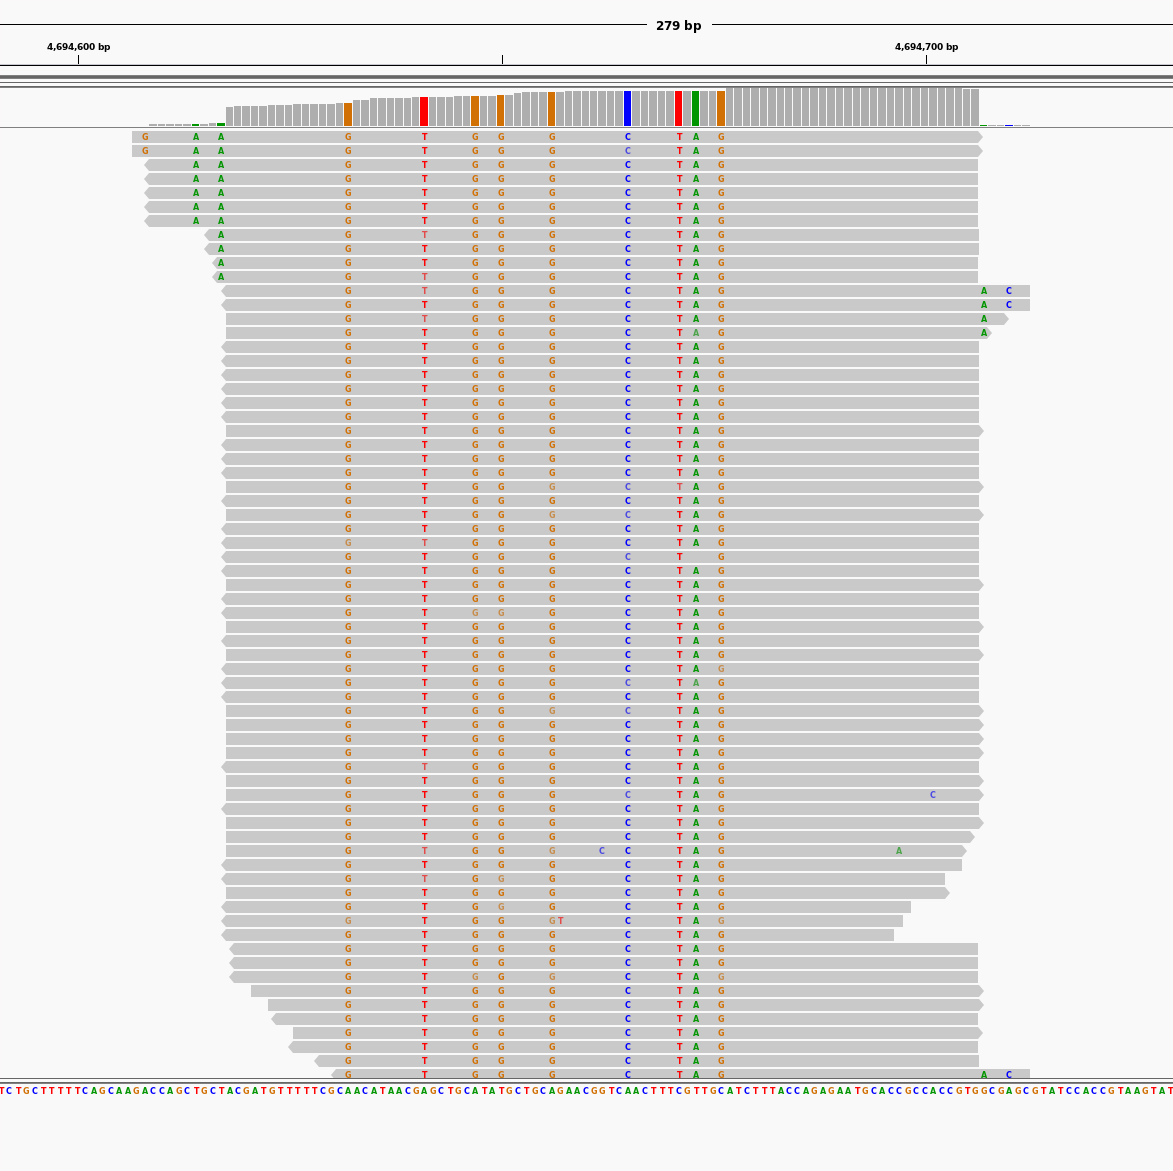
\includegraphics[width=0.35\textheight]{bacillus_reads.png}
\caption{Alignment of short reads from pEU23\_OXA to the \textit{Bacillus cereus}. The reads map with a few SNPs which are colored. The reads also don't overlap.}
\label{figure:bacillus_reads}
\end{figure}
Since some samples of the morbidostat showed \textit{Bacillus cereus} contaminations we analyzed the short reads of the ESBL \textit{E. coli} stocks. Table \ref{table:bacillus_reads} shows how many Illumina reads of the stocks mapped to \textit{Bacillus cereus ATCC 14579} and to the ESBL \textit{E. coli} reference genome produced with hybrid-assembling. 
Around 0.44 \% of all Illumina reads mapped to \textit{Bacillus cereus ATCC 14579}. In Figure \ref{figure:bacillus_reads} one region of an alignment of the Illumina reads to the \textit{Bacillus cereus} genome is shown. We could see that Illumina reads only mapped to very certain regions of the genome of \textit{Bacillus cereus} without overlapping and with a variation of a few bases. Because the reads were not overlapping and they did not map with an identity of 100\%, the stocks were not contaminated. Also the hybrid-assembly of the reference genome did not show any contigs with \textit{Bacillus cereus} sequences.

The outcome of mapping the Illumina reads to \textit{Bacillus cereus} and ESBL \textit{E. coli} for the morbidostat samples is shown in Table \ref{table:bacillus_reads_samples}. Looking at the percentage of how many reads mapped to \textit{Bacillus cereus} showed that two groups exist. Ether 60 \% or more, implying that the samples were contaminated, or only 0.48 \%  mapped to \textit{Bacillus cereus} implying that those samples were not contaminated. From all morbidostat samples 12 samples had fewer reads than 0.48 \% and were not contaminated. 

\begin{table}[H]
	\begin{tabularx}{\linewidth}{|LccLLLL|}
		\hline
		Experiment & Vial & Sample & Total reads & Reads mapped to \textit{Bacillus cereus} & Reads mapped to \textit{E. coli} & \% of reads mapped to \textit{Bacillus cereus} \\ \hline
		01         & 1    & 1      & 6490750     & 4967611                         & 272289                  & 76.53                                \\ \hline
		01         & 2    & 1      & 7601839     & 6001106                         & 418578                  & 78.94                                \\ \hline
		01         & 3    & 1      & 2940556     & 13976                           & 2934902                 & 0.48                                 \\ \hline
		01         & 4    & 1      & 8167777     & 6150829                         & 281584                  & 75.31                                \\ \hline
		01         & 5    & 1      & 5606842     & 4089104                         & 178462                  & 72.93                                \\ \hline
		01         & 9    & 1      & 5636939     & 4466280                         & 268813                  & 79.23                                \\ \hline
		01         & 10   & 1      & 4935808     & 22368                           & 4928816                 & 0.45                                 \\ \hline
		02         & 1    & 1      & 6152378     & 26815                           & 6143228                 & 0.44                                 \\ \hline
		02         & 2    & 1      & 6926506     & 5180940                         & 291927                  & 74.80                                \\ \hline
		02         & 3    & 1      & 5142535     & 24909                           & 5136761                 & 0.48                                 \\ \hline
		02         & 3    & 2      & 6196309     & 4694898                         & 279679                  & 75.77                                \\ \hline
		02         & 4    & 1      & 4923087     & 22342                           & 4915639                 & 0.45                                 \\ \hline
		02         & 4    & 2      & 4589212     & 20628                           & 4582915                 & 0.45                                 \\ \hline
		02         & 5    & 1      & 4298753     & 17870                           & 4292083                 & 0.42                                 \\ \hline
		02         & 5    & 2      & 5189054     & 22772                           & 5181923                 & 0.44                                 \\ \hline
		02         & 7    & 1      & 5167596     & 22583                           & 5159028                 & 0.44                                 \\ \hline
		02         & 7    & 2      & 4976635     & 3015316                         & 107767                  & 60.59                                \\ \hline
		02         & 8    & 1      & 4356280     & 19067                           & 4350598                 & 0.44                                 \\ \hline
		02         & 8    & 2      & 4186125     & 18526                           & 4181356                 & 0.44                                 \\ \hline
		02         & 9    & 1      & 4182681     & 18487                           & 4176477                 & 0.44                                 \\ \hline
		02         & 10   & 1      & 3809536     & 2576863                         & 136340                  & 67.64                                \\ \hline
	\end{tabularx}
	\caption{Illumina reads from every morbidostat sample mapped to to a \textit{Bacillus cereus} from NCBI \cite{noauthor_bacillus_nodate} and the \textit{E.coli} reference genome produced with  hybrid-assembling.}
	\label{table:bacillus_reads_samples}
\end{table}

\subsection{Grow curves and injected concentrations for cultures grown with the morbidostat}
\begin{figure}[H]
	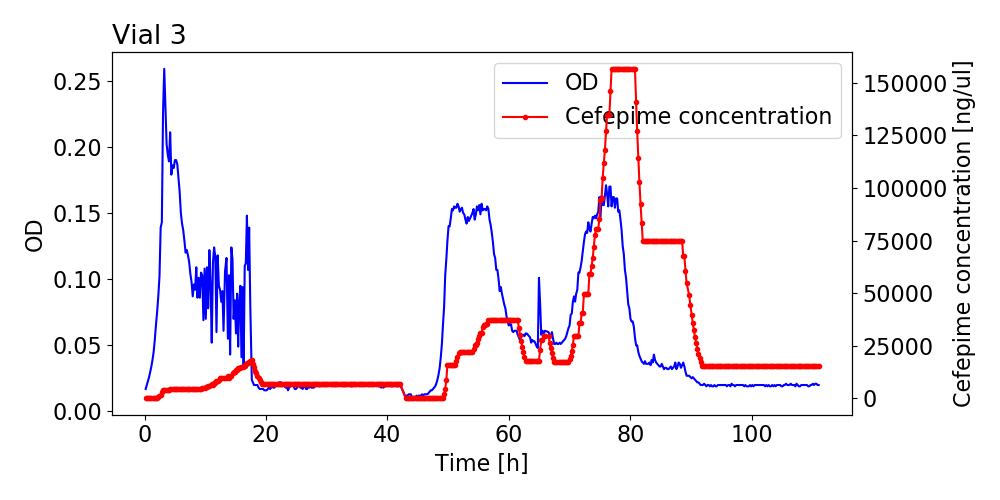
\includegraphics[width=0.5\textwidth]{01_vial_3.png}
	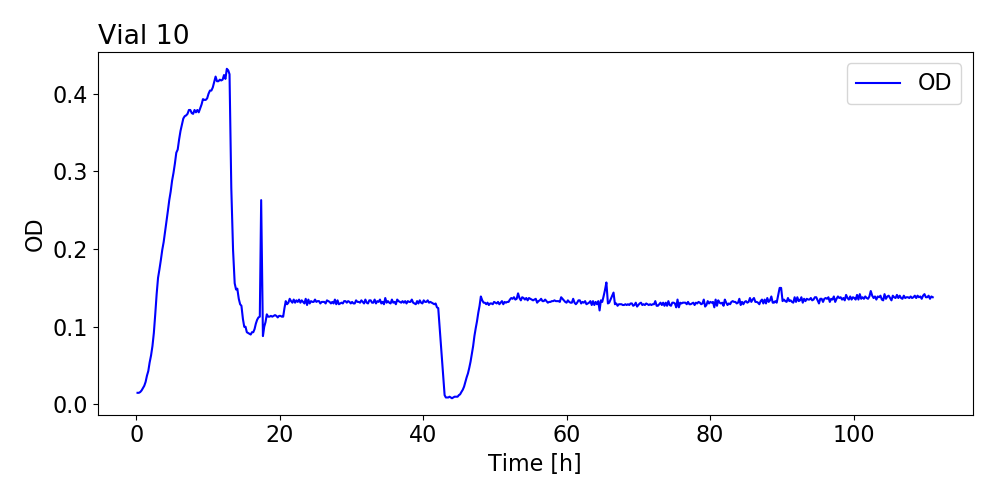
\includegraphics[width=0.5\textwidth]{01_vial_10.png}
	\caption{Grow curves and cefepime concentration in the vials which were not contaminated from experiment 01.}
	\label{figure:01_vials}
\end{figure}

\begin{figure}[h]	
	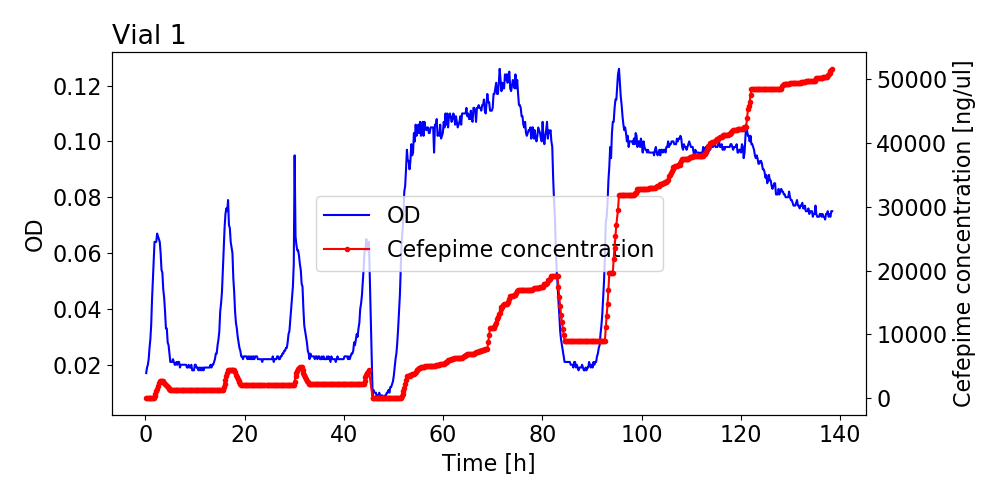
\includegraphics[width=0.5\textwidth]{02_vial_1.png}
	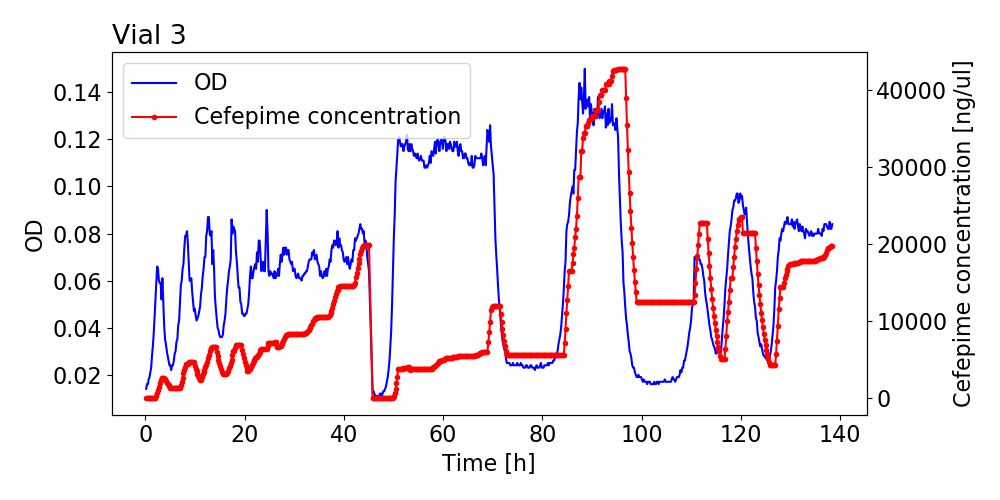
\includegraphics[width=0.5\textwidth]{02_vial_3.png}
	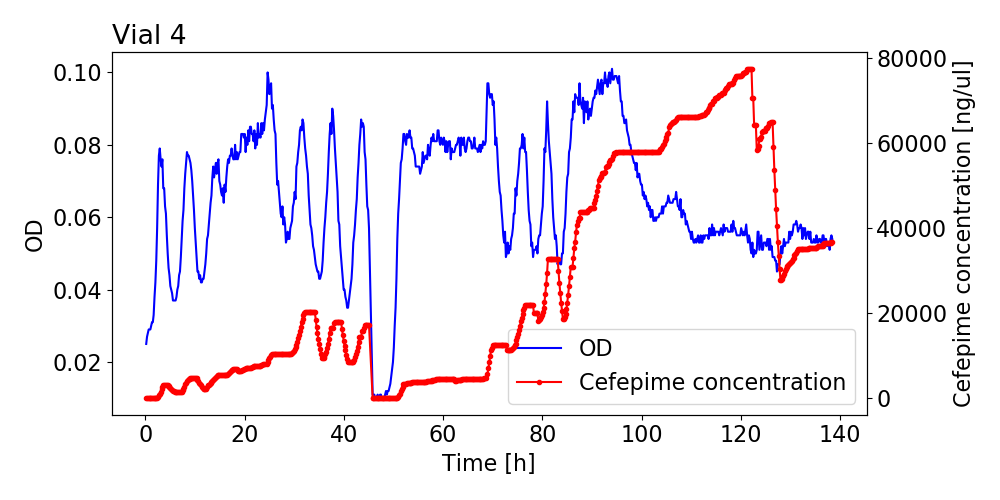
\includegraphics[width=0.5\textwidth]{02_vial_4.png}
	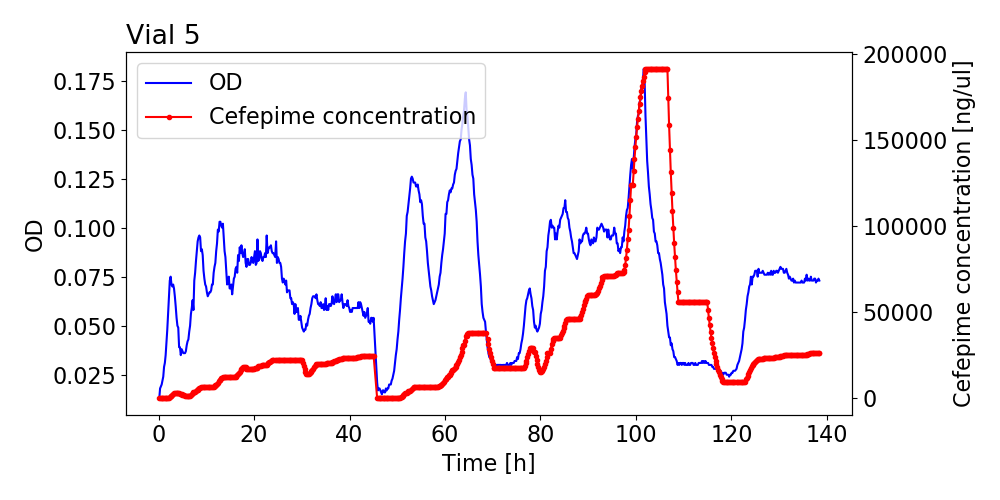
\includegraphics[width=0.5\textwidth]{02_vial_5.png}	
	\caption{Grow curves and cefepime concentration in the vials which were not contaminated from experiment 01.}
	\label{figure:02_vials}
\end{figure}
Figure \ref{figure:01_vials} and Figure \ref{figure:02_vials} show the recorded ODs and the the cefepime concentration in the vials from the morbidostat experiment 01 (Figure \ref{figure:01_vials}) and 02 (Figure \ref{figure:02_vials}). From both experiments only the vials with no contamination are shown. After 45 hours 200 \textmu of the cell suspensions were transferred into a new vial with 18 mL diluted media. This is causing the abrupt drop of ODs. In vial 3 from the 01 experiment the OD measurements wher very noisy at the beginning which was caused by an air cone coming from high stirring with the magnetic stirrer. After 20 hours the stirring was reduced which eliminated the noise. For vial 10 the mode was set to record growth rate instead of fixed OD. The mode was changed to fixed OD after 15 hours. 
In general the feedback worked really well. The left Figure \ref{figure:vial_3_area} shows the first 45 hours for vial 3 from experiment 02. Drug injection took place after the drug\_dilution\_threshold was reached. After that the cefepime concentration was continuously increased until the cells started to die. The cefepime concentration which was necessary to kill the majority of the cells was stored. Then the feedback diluted the cultures with media unitl half of the deadly concentration was reached. After that no injections took place until the culture started to grow again. The result of the feedback was that the OD was kept pretty steady but the cefepime concentration continuously increased. The deadly cefepime concentration after 40 hours of culturing was already four fold higher than at the beginning. 
\begin{figure}[H]
	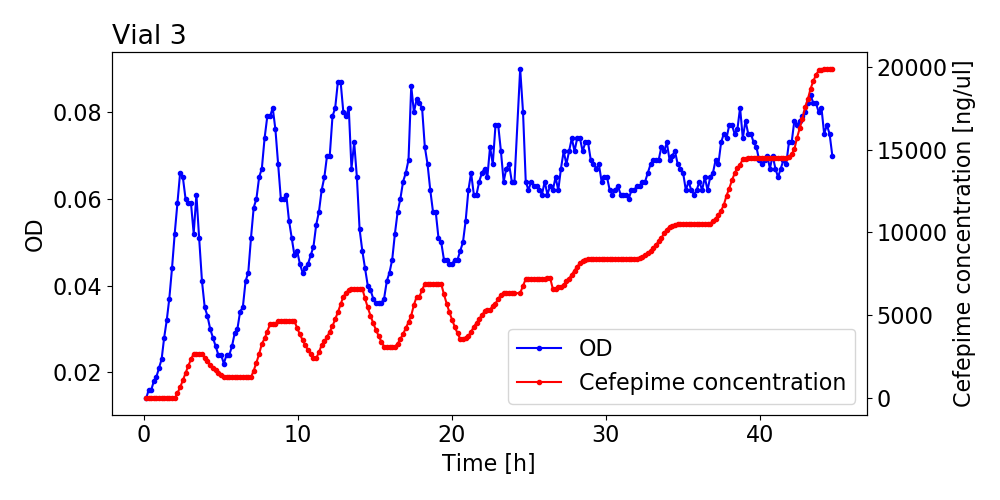
\includegraphics[width=0.5\textwidth]{vial_3_area.png}
	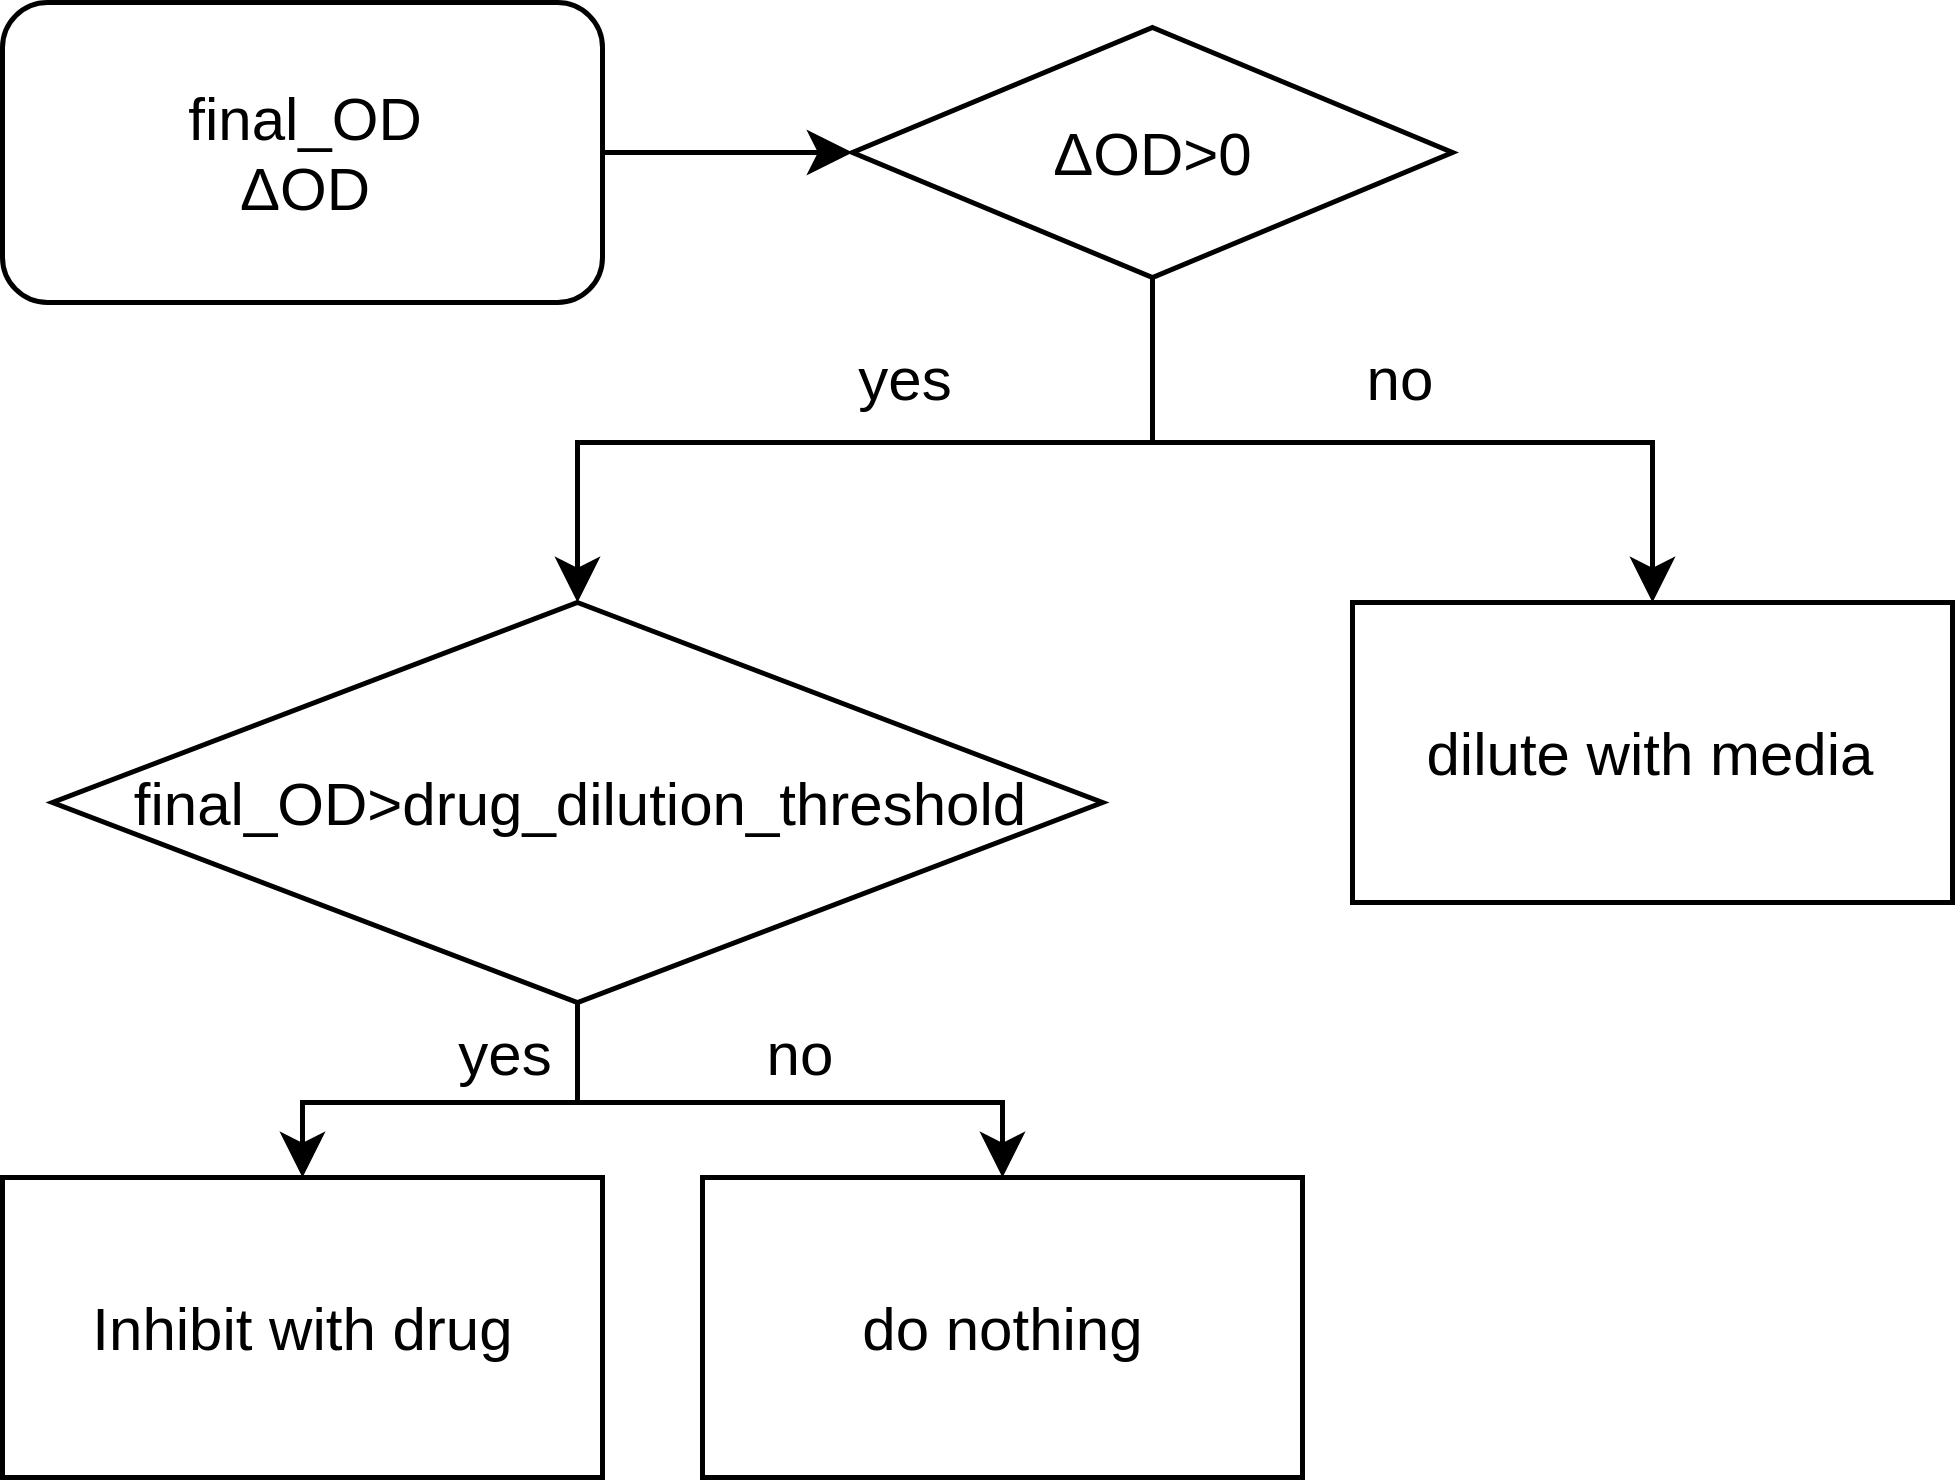
\includegraphics[width=0.5\textwidth]{feedback.png}
	\caption{Left: First 45 hours from vial 3 of experiment 02. Right: Feedback algorithm deciding over drug injection.}
	\label{figure:vial_3_area}
\end{figure}
\subsection{MIC of the strains used for culturing with the morbidostat}
The MICs of the strains used for the experiment 01 and 02 are shown in Figure \ref{figure:mic_ogs}
\begin{figure}[H]
	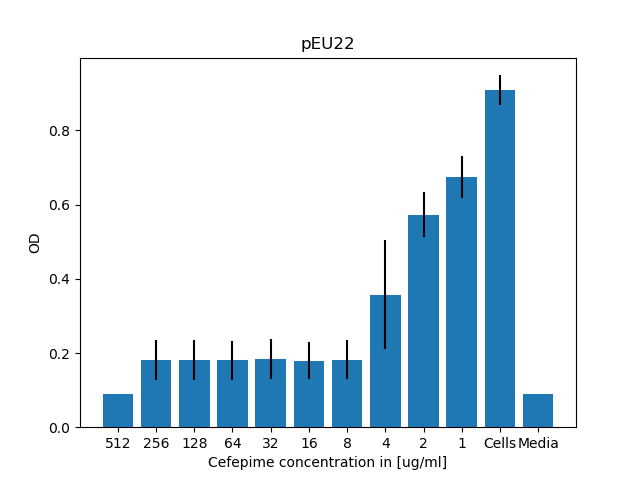
\includegraphics[width=0.3\textwidth]{22a_cef.png}
	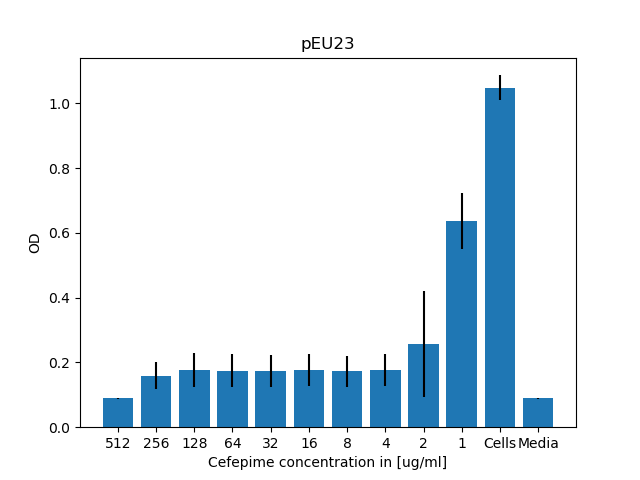
\includegraphics[width=0.3\textwidth]{23a_cef.png}
	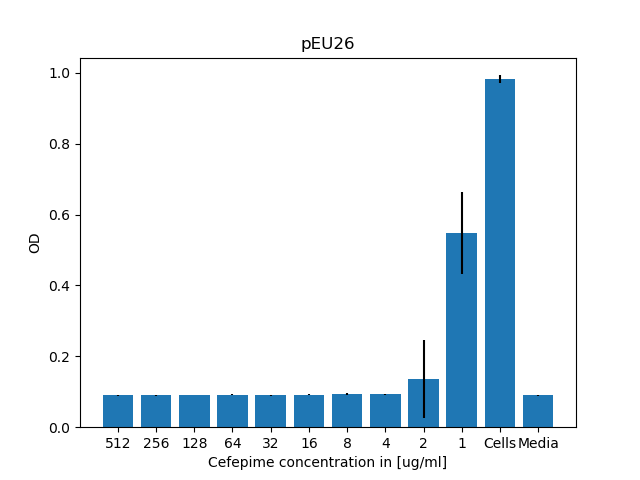
\includegraphics[width=0.3\textwidth]{26a_cef.png}
	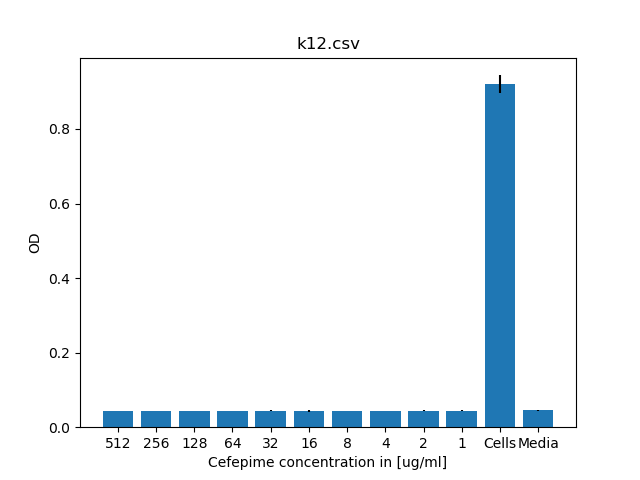
\includegraphics[width=0.3\textwidth]{k12.png}
	\caption{MICs of the strains used for the experiment 01 and 02.}
	\label{figure:mic_ogs}
\end{figure}
\begin{figure}[H]
	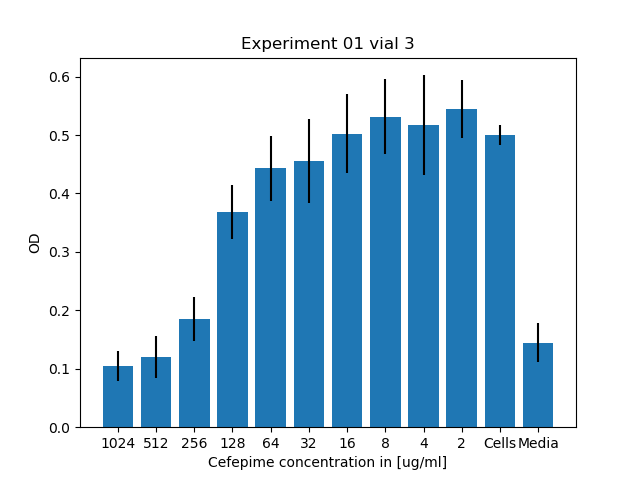
\includegraphics[width=0.3\textwidth]{vial3_OXA_patient25.png}
	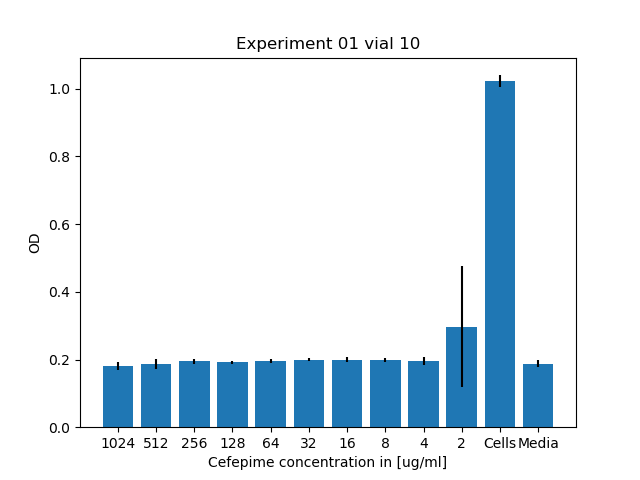
\includegraphics[width=0.3\textwidth]{vial9_OXA_patient25_dilution_control.png}
	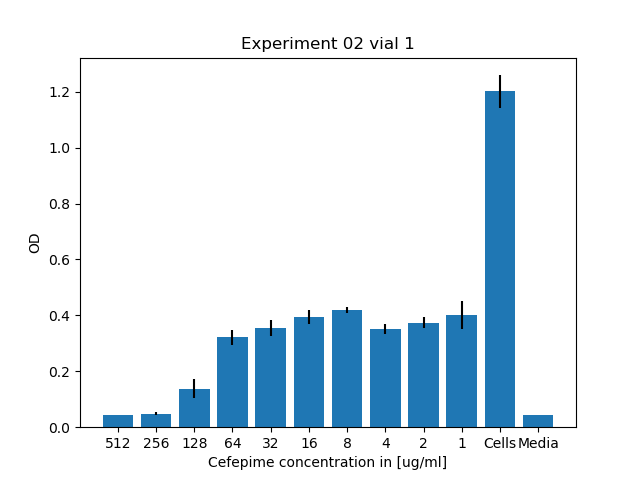
\includegraphics[width=0.3\textwidth]{v1.png}
	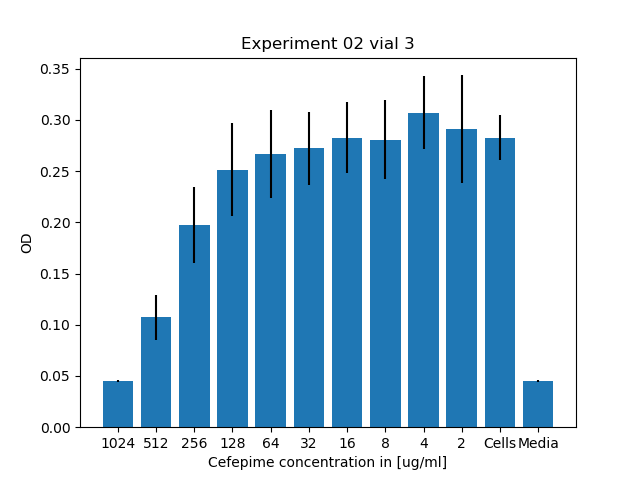
\includegraphics[width=0.3\textwidth]{v3.png}
	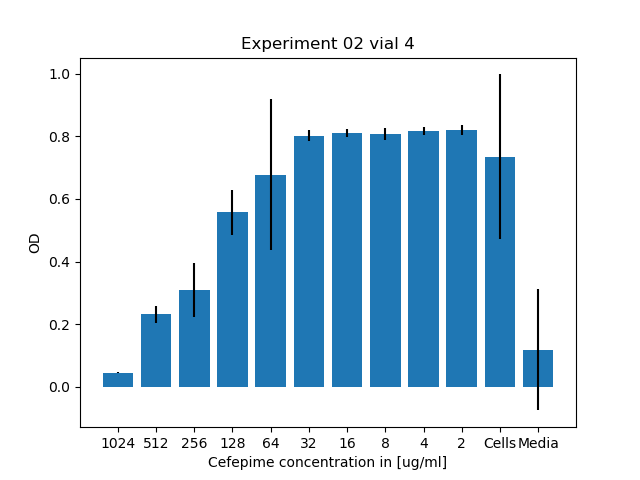
\includegraphics[width=0.3\textwidth]{v4.png}
	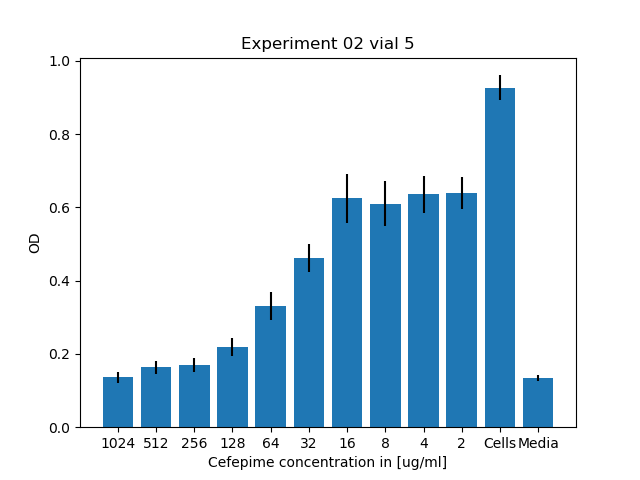
\includegraphics[width=0.3\textwidth]{v5.png}
	\label{figure:mics_finish}
	\caption{MICs of the samples from the last sample day of the experiment 01 and 02.}
\end{figure}
\subsection{SNPs of experiment 01}
\subsubsection{Vial 3}
No SNPs in the samples of vial 3 were found.
\subsubsection{Vial 10}
Even though vial 10 was cultured with the fixed OD mode, one SNP was found in the samples. The position of the SNP is shown in Table \ref{table:01_10} and their annotation in Table \ref{table:01_10_ann}.
\begin{table}[H]
	\begin{tabularx}{\linewidth}{|cccLL|}
		\hline
		\#SNP & Contig & Position & \multicolumn{2}{l|}{Nucleotide in Sample:} \\
		&        &          & 0         & \multicolumn{1}{l|}{1}    \\ \hline
		1 & 0 & 3403729 & G & C \\ \hline
	\end{tabularx}
	\label{table:01_10}
	\caption{Positions of SNPs in the samples of vial 10 experiment 01.}
\end{table} 
\begin{table}[H]
	\begin{tabularx}{\linewidth}{|ccLLcc|}
		\hline
		\#SNP & Gene          & Product                           & Type and position & \multicolumn{2}{l|}{Amino acid Sample:} \\
		&               &                                   &                   & 0                  & 1                  \\ \hline
	1 & \textit{tomB\_1} & Hha toxicity modulator TomB & Silent, 43 & I & V \\ \hline
	
	\end{tabularx}
	\caption{Genes affected by the SNPs found in the samples of vial 10 experiment 02.}
	\label{table:01_10_ann}
\end{table}
\subsection{SNPs of experiment 02}
\subsubsection{Vial 1}
No SNPs were found in the samples of this vial.
\subsubsection{Vial 3}
One SNP was found in the samples of vial 3 which is shown in Table \ref{table:3_02}. Interestingly this mutation affects the kanamycin resistance gene of the vector. The change of amino acid caused by the SNP is shown in Table \ref{table:02_3_ann}.
\begin{table}[H]
	\begin{tabularx}{\linewidth}{|cccLL|}
		\hline
		\#SNP & Contig & Position & \multicolumn{2}{l|}{Nucleotide in Sample:} \\
		&        &          & 0         & \multicolumn{1}{l|}{1}    \\ \hline
		1 & 1 & 4290 & G & T \\ \hline
	\end{tabularx}
	\label{table:3_02}
	\caption{Positions of SNPs in the samples of vial 3 experiment 02.}
\end{table} 
\begin{table}[H]
	\begin{tabularx}{\linewidth}{|ccLLcc|}
		\hline
		\#SNP & Gene          & Product                           & Type and position & \multicolumn{2}{l|}{Amino acid Sample:} \\
		&               &                                   &                   & 0                  & 1                  \\ \hline
		1 & \textit{neoR/kanR} & Kanamycin resistance & Missense, 204 & G & V \\ \hline
		
	\end{tabularx}
	\label{table:02_3_ann}
	\caption{Genes affected by the SNPs found in the samples of vial 10 experiment 01.}
\end{table}
\subsubsection{Vial 4}
Two SNPs were found for the samples of vial 4 shown in Table \ref{table:02_v4} and the affected genes in Table \ref{table:02_v4_ann}.
\begin{table}[H]
	\begin{tabularx}{\linewidth}{|cccLLL|}
		\hline
		\#SNP & Contig & Position & \multicolumn{3}{l|}{Nucleotide in Sample:} \\
		&        &          & 0     & 1     & \multicolumn{1}{l|}{2}    \\ \hline
		1 & 1 & 2526   & T & T & A \\ \hline
		2 & 0 & 347328 & C & C & T \\ \hline
	\end{tabularx}
	\label{table:02_v4}
	\caption{Positions of SNPs in the samples of vial 4 experiment 02.}
\end{table}

\begin{table}[H]
	\begin{tabularx}{\linewidth}{|ccLLccc|}
		\hline
		\#SNP & Gene          & Product                                  & Type and position in gene      & \multicolumn{3}{l|}{Amino acid in Sample:} \\
		&               &                                          &                        & 0   & 1               & 2               \\ \hline
		1 & \textit{bla}  & Beta-lactamase CTX-M-1                  & Missense, 289 & V & V & D \\ \hline
		2 & \textit{ompR} & Transcriptional regulatory protein OmpR & Nonsense, 67  & R & R & * \\ \hline
	\end{tabularx}
	\caption{Genes affected by the SNPs found in the samples of vial 4 experiment 02.}
	\label{table:02_v4_ann}
\end{table}
\subsubsection{Vial 5}
Three SNPs were found for the samples of vial 5. SNPs are shown Table \ref{table:02_v5}, annotations in Table \ref{table:02_v5_ann}.
\begin{table}[H]
	\begin{tabularx}{\linewidth}{|cccLLL|}
		\hline
		\#SNP & Contig & Position & \multicolumn{3}{l|}{Nucleotide in Sample:} \\
		&        &          & 0     & 1     & \multicolumn{1}{l|}{2}    \\ \hline
		1 & 0 & 1570984 & C & C & T \\ \hline
		2 & 0 & 668881  & A & T & A \\ \hline
		3 & 0 & 2898640 & G & G & - \\ \hline
	\end{tabularx}
	\label{table:02_v5}
	\caption{Positions of SNPs in the samples of vial 5 experiment 02.}
\end{table}

\begin{table}[H]
	\begin{tabularx}{\linewidth}{|ccLLccc|}
		\hline
		\#SNP & Gene          & Product                                  & Type and position in gene      & \multicolumn{3}{l|}{Amino acid in Sample:} \\
		&               &                                          &                        & 0   & 1               & 2               \\ \hline
		1 & \textit{ompC\_1} & Outer membrane protein C         & Silent, 8              & L & L & L \\ \hline
		2 & \textit{rpoD}    & RNA polymerase sigma factor RpoD & Missense, 594             & L & Q & L \\ \hline
		3 & \textit{ompF}    & Outer membrane protein F         & Frameshift, 319 & G & G & A \\ \hline
	\end{tabularx}
	\caption{Genes affected by the SNPs found in the samples of vial 5 experiment 02.}
	\label{table:02_v5_ann}
\end{table}
